\documentclass[aspectratio=169]{beamer}

\usepackage{ccicons}
\usepackage{fontspec}
\usepackage{listings}
\usepackage{tikz}
\usepackage{svg}

\definecolor{uclablue}{RGB}{39,116,174}
\definecolor{uclagold}{RGB}{255,179,0}

\definecolor{ubcorange}{RGB}{158, 66, 37}

\definecolor{cugold}{RGB}{207, 184, 124}
\definecolor{cudarkgray}{RGB}{86, 90, 92}

\definecolor{solarizedred}{RGB}{220, 50, 47}
\definecolor{solarizedblue}{RGB}{38, 139, 210}
\definecolor{solarizedgreen}{RGB}{133, 153, 0}
\definecolor{solarizedpurple}{RGB}{108, 113, 196}
\definecolor{solarizedmagenta}{RGB}{211, 54, 130}

\definecolor{pantone655}{RGB}{0, 42, 92}
\definecolor{pantone7453}{RGB}{123, 164, 217}
\definecolor{pantone633}{RGB}{0, 139, 176}
\definecolor{pantone7492}{RGB}{218, 229, 205}

\colorlet{primarycolor}{pantone655}
\colorlet{secondarycolor}{pantone7453}


\usetikzlibrary{
  arrows,
  arrows.meta,
  automata,
  backgrounds,
  calc,
  chains,
  decorations.pathreplacing,
  fit,
  intersections,
  matrix,
  overlay-beamer-styles,
  positioning,
  shapes,
  shapes.multipart,
  tikzmark,
}
\usetikzmarklibrary{listings}

\hypersetup{
  colorlinks=true,
  urlcolor=cudarkgray,
}

\setbeamercolor{frametitle}{fg=primarycolor}
\setbeamercolor{structure}{fg=primarycolor}
\setbeamercolor{enumerate item}{fg=black}
\setbeamercolor{itemize item}{fg=black}
\setbeamercolor{itemize subitem}{fg=black}

\setbeamersize{text margin left=26.6mm}
\addtolength{\headsep}{2mm}

\setbeamertemplate{navigation symbols}{}
\setbeamertemplate{headline}{}
\setbeamertemplate{footline}{}
\setbeamertemplate{itemize item}{\color{black}}
\setbeamertemplate{itemize items}[circle]

\setbeamertemplate{footline}{
  \begin{tikzpicture}[remember picture,
                      overlay,
                      shift={(current page.south west)}]
    \node [black!50, inner sep=2mm, anchor=south east]
          at (current page.south east) {\footnotesize \insertframenumber};
  \end{tikzpicture}
}

\setsansfont{Inter}[Scale=MatchLowercase]
\setmonofont{Hack}[Scale=MatchLowercase]

\makeatletter
\newcommand\version[1]{\renewcommand\@version{#1}}
\newcommand\@version{}
\def\insertversion{\@version}

\newcommand\lecturenumber[1]{\renewcommand\@lecturenumber{#1}}
\newcommand\@lecturenumber{}
\def\insertlecturenumber{\@lecturenumber}
\makeatother

\setbeamertemplate{title page}
{
  \begin{tikzpicture}[remember picture,
                      overlay,
                      shift={(current page.south west)},
                      background rectangle/.style={fill=pantone655},
                      show background rectangle]
    \node [anchor=west, align=left, inner sep=0, text=white]
          (lecturenumber) at (\paperwidth / 6, \paperheight * 3 / 4)
          {\Large Lecture \insertlecturenumber};
    \node [inner sep=0, align=left, text=white, node distance=0,
          above left=of lecturenumber, anchor=south west, yshift=2mm]
          {\Large ECE 344: Operating Systems};
    \node (title) [inner sep=0, anchor=west, align=left, text=white,
                   text width=30em]
          at (\paperwidth / 6, \paperheight / 2)
          {{\bfseries \Huge \inserttitle{}}};
    \node [inner sep=0, align=right, text=white, node distance=0,
          below right=of title, anchor=north east, yshift=-1mm]
          {{\footnotesize \ttfamily \insertversion}};
    \node [inner sep=0, text=white, align=left, anchor=west]
          (author) at (\paperwidth / 6, \paperheight / 4)
          {\insertauthor};
    \node [text=white, inner sep=0, align=left, node distance=0,
           below left=of author, anchor=north west, yshift=-2mm]
          {\insertdate};
    \node [align=right, anchor=south east, inner sep=2mm, text=white]
          (license) at (\paperwidth, 0)
          {\footnotesize This  work is licensed under a
           \href{http://creativecommons.org/licenses/by-sa/4.0/}
                {\color{pantone7453} Creative Commons Attribution-ShareAlike 4.0
                 International License}};
    \node [text=white, inner sep=0, align=right, node distance=0,
           above right=of license, anchor=south east, xshift=-2mm]
          {\Large \ccbysa};
  \end{tikzpicture}
}

\tikzset{
  >=Straight Barb[],
  shorten >=1pt,
  initial text=,
}

\lstset{
  basicstyle=\footnotesize\ttfamily,
  language=C,
  escapechar=@,
  commentstyle=\color{black!50},
}


\lecturenumber{19}
\title{Single-Level Page Tables}
\version{1.0.1}
\author{Jon Eyolfson}
\date{October 24, 2021}

\begin{document}
  \begin{frame}[plain, noframenumbering]
    \titlepage
  \end{frame}

  \begin{frame}
    \frametitle{Virtualization Fools Something into Thinking it Has All Resources}

    \begin{columns}[c]
      \column{0.5\textwidth}
      \flushright
    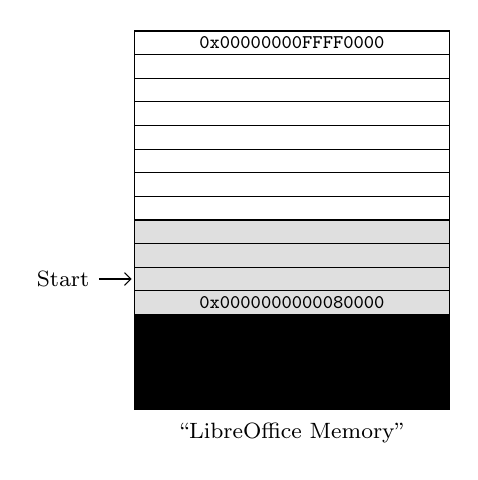
\begin{tikzpicture}
      \node [align=center] at (2, 0) {\footnotesize ``LibreOffice Memory''};
      \draw [fill=black] (0, 0.3) rectangle (4, 1.5);
      \draw [fill=black!12.5] (0, 1.5) rectangle (4, 2.7);
      \node [align=center] at (2, 1.65) {\scriptsize \ttfamily 0x0000000000080000};
      \node [align=center] at (2, 4.95) {\scriptsize \ttfamily 0x00000000FFFF0000};
      \foreach \i in {1, ..., 16}
      {
        \draw (0, 0.3 * \i) rectangle (4, \i * 0.3 + 0.3);
      }

      \draw [->] (-0.45, 1.95) -- (0, 1.95) node [pos=0, anchor=east] {\footnotesize Start};
    \end{tikzpicture}
      \column{0.5\textwidth}
      \flushleft
    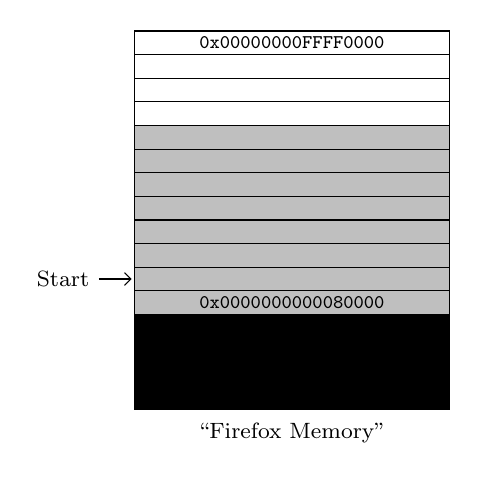
\begin{tikzpicture}
      \node [align=center] at (2, 0) {\footnotesize ``Firefox Memory''};
      \draw [fill=black] (0, 0.3) rectangle (4, 1.5);
      \draw [fill=black!25] (0, 1.5) rectangle (4, 3.9);
      \node [align=center] at (2, 1.65) {\scriptsize \ttfamily 0x0000000000080000};
      \node [align=center] at (2, 4.95) {\scriptsize \ttfamily 0x00000000FFFF0000};
      \foreach \i in {1, ..., 16}
      {
        \draw (0, 0.3 * \i) rectangle (4, \i * 0.3 + 0.3);
      }

      \draw [->] (-0.45, 1.95) -- (0, 1.95) node [pos=0, anchor=east] {\footnotesize Start};
    \end{tikzpicture}
    \end{columns}
  \end{frame}

  \begin{frame}
    \frametitle{Virtual Memory Checklist}

    \begin{itemize}
      \item [$\square$] Multiple processes must be able to co-exist
      \item [$\square$] Processes are not aware they are sharing physical memory
      \item [$\square$] Processes cannot access each others data (unless allowed explicitly)
      \item [$\square$] Performance close to using physical memory
      \item [$\square$] Limit the amount of fragmentation (wasted memory)
    \end{itemize}
  \end{frame}

  \begin{frame}
    \frametitle{Memory Management Unit (MMU)}

    Maps virtual address to physical address

    \hspace{2em} Also checks permissions

    \vspace{2em}

    One technique is to divide memory up into fixed-size pages (typically 4096 bytes)

    \hspace{2em} A page in virtual memory is called a page

    \hspace{2em} A page in physical memory is called a frame
  \end{frame}

  \begin{frame}
    \frametitle{Segmentation or Segments are Coarse Grained}

    Divide the virtual address space into segments for: code, data, stack, and heap

    \hspace{2em} Note: this looks like an ELF file, large sections of memory with permissions

    \vspace{2em}

    Each segment is a variable size, and can be dynamically resized

    \hspace{2em} This is an old legacy technique that's no longer used

    \vspace{2em}

    Segments can be large and very costly to relocate

    \hspace{2em} It also leads to fragmentation (gaps of unused memory)

    \vspace{2em}

    No longer used in modern operating systems
  \end{frame}

  \begin{frame}
    \frametitle{Segmentation Details}

    Each segment contains a: base, limit, and permissions

    \hspace{2em} You get a physical address by using: \texttt{segment selector:offset}

    \vspace{2em}

    The MMU checks that your offset is within the limit (size)

    \hspace{2em} If it is, it calculates base + offset, and does permission checks

    \hspace{4em} Otherwise, it's a segmentation fault

    \vspace{2em}

    For example 0x1:0xFF with segment 0x1 base = 0x2000, limit = 0x1FF

    \hspace{2em} Translates to 0x20FF

    \vspace{2em}

    Note: Linux sets every base to 0, and limit to the maximum amount
  \end{frame}

  \begin{frame}
    \frametitle{You Typically Do Not Use All 64 Virtual Address Bits}

    CPUs may have different levels of virtual addresses you can use

    \hspace{2em} Implementation ideas are the same

    \vspace{2em}

    We'll assume a 39 bit virtual address space used by RISC-V and other
    architectures

    \hspace{2em} Allows for 512 GiB of addressable memory (called Sv39)

    \vspace{2em}

    Implemented with a page table indexed by Virtual Page Number (VPN)

    \hspace{2em} Looks up the Physical Page Number (PPN)
  \end{frame}

  \begin{frame}
    \frametitle{The Page Table Translates Virtual to Physical Addresses}

    \begin{center}
      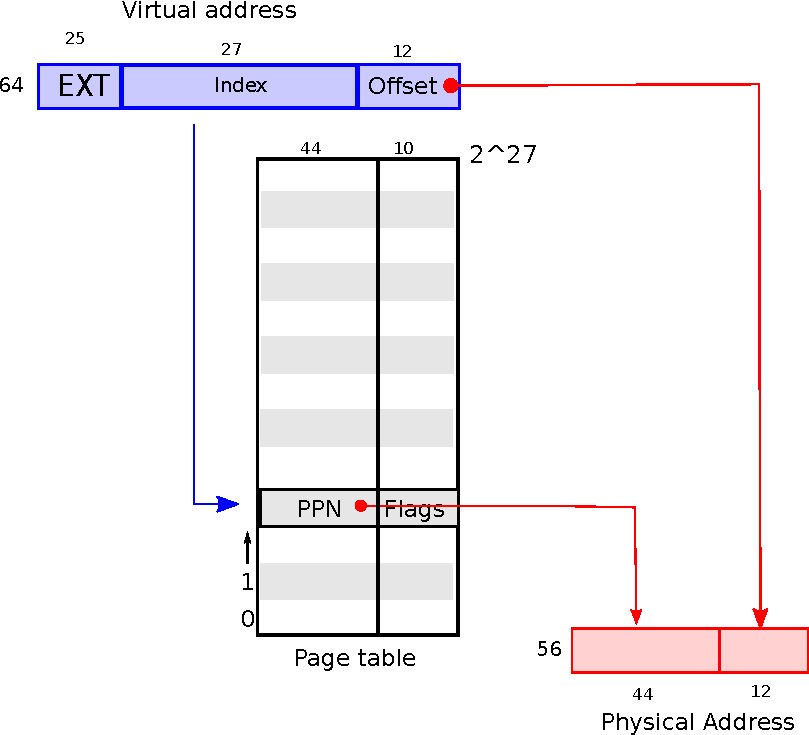
\includegraphics[scale=0.5]{riscv_address.pdf}
    \end{center}

    © MIT \url{https://github.com/mit-pdos/xv6-riscv-book/}
  \end{frame}

  \begin{frame}
    \frametitle{The Kernel Handles Translating Virtual Addresses}

    Considering the following page table:

    \begin{center}
    {\ttfamily
    \begin{tabular}{ll}
      VPN  & PPN  \\
      0x0 & 0x1 \\
      0x1 & 0x4 \\
      0x2 & 0x3 \\
      0x3 & 0x7 \\
    \end{tabular}}
    \end{center}

    We would get the following virtual $\rightarrow$ physical address translations:

    \begin{center}
    \texttt{0x0AB0} $\rightarrow$ \texttt{0x1AB0}
    
    \texttt{0x1FA0} $\rightarrow$ \texttt{0x4FA0}

    \texttt{0x2884} $\rightarrow$ \texttt{0x3884}

    \texttt{0x32D0} $\rightarrow$ \texttt{0x72D0}
    \end{center}
  \end{frame}

  \begin{frame}
    \frametitle{Page Translation Example Problem}

    Assume you have a 8-bit virtual address, 10-bit physical address

    \hspace{2em} and each page is 64 bytes

    \begin{itemize}
      \item How many virtual pages are there? \onslide<2->{$\mathsf{\frac{2^8}{2^6} = 4}$}
      \item How many physical pages are there? \onslide<2->{$\mathsf{\frac{2^{10}}{2^6} = 16}$}
      \item How many entries are in the page table? \onslide<2->{$\mathsf{4}$}
      \item Given the page table is \texttt{{[0x2, 0x5, 0x1, 0x8]}}

            \hspace{2em} what's the physical address of \texttt{0xF1}?

            \onslide<2->{\texttt{0x231}}
    \end{itemize}
  \end{frame}

  \begin{frame}
    \frametitle{The Page Table Entry (PTE) Also Stores Flags in the Lower Bits}

    \begin{center}
      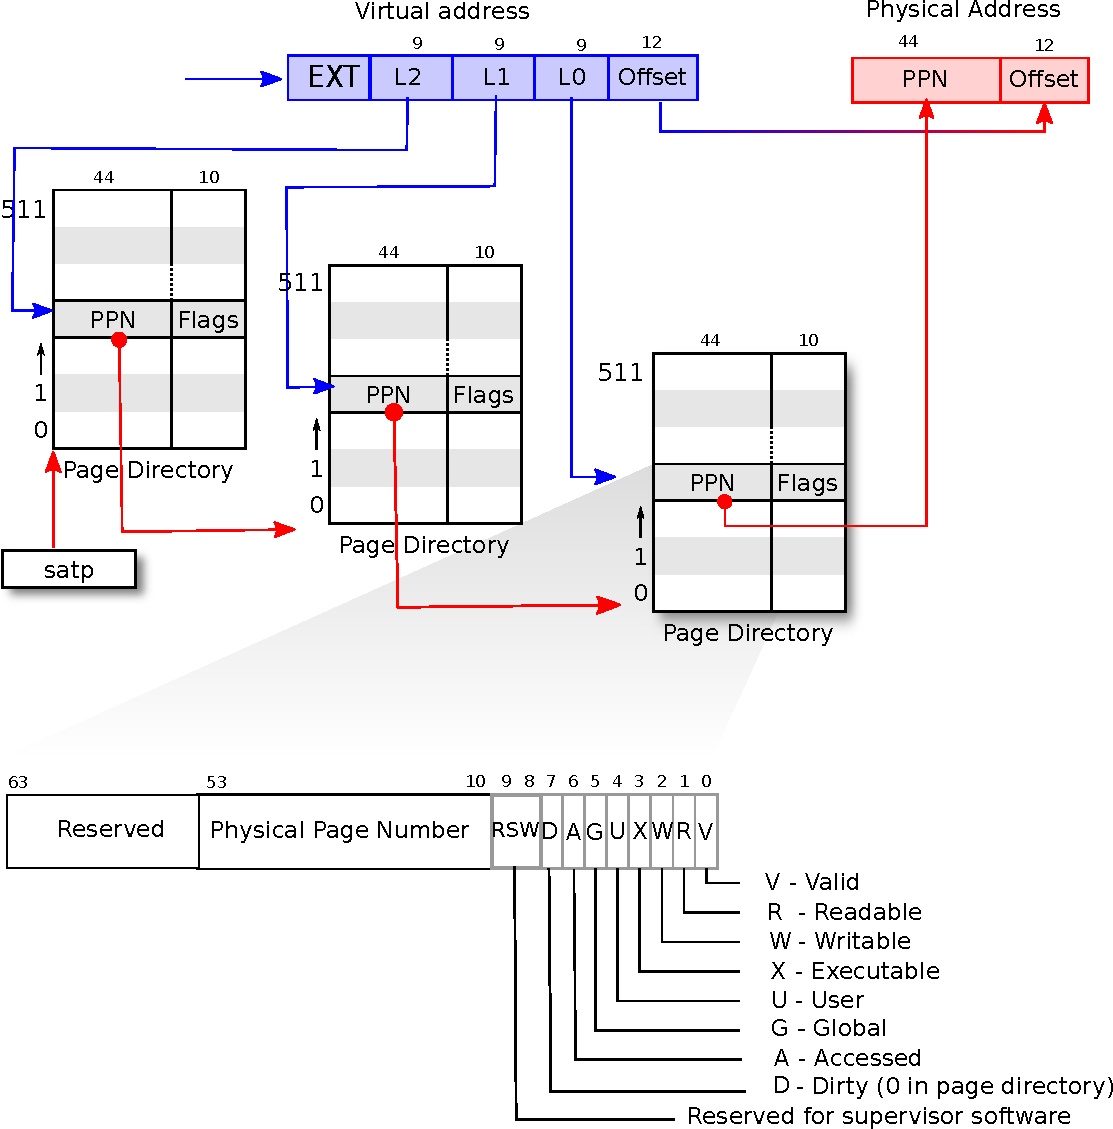
\includegraphics[scale=0.5, clip, trim=0cm 0cm 0cm 13cm]{riscv_pagetable.pdf}
    \end{center}

    © MIT \url{https://github.com/mit-pdos/xv6-riscv-book/}

    \vspace{2em}

    The MMU which uses the page table checks these flags

    \hspace{2em} We'll focus on the first 5 flags
  \end{frame}

  \begin{frame}
    \frametitle{Each Process Gets Its Own Virtual Address Space}

    \begin{center}
      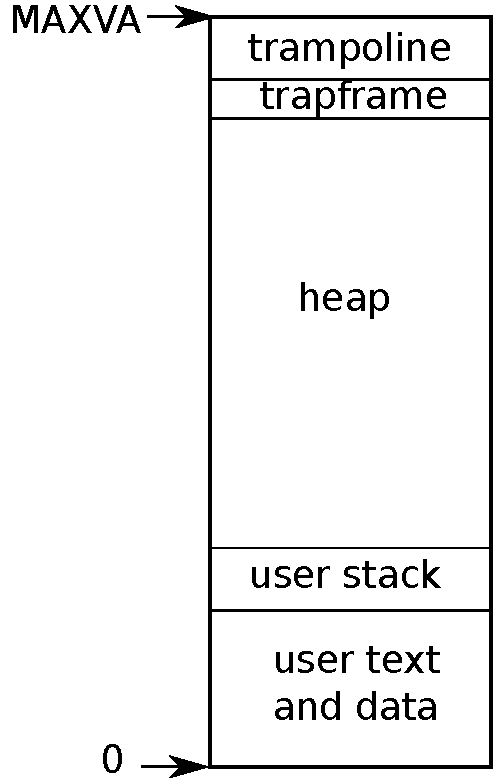
\includegraphics[scale=0.4]{as.pdf}
    \end{center}

    © MIT \url{https://github.com/mit-pdos/xv6-riscv-book/}
  \end{frame}

  \begin{frame}
    \frametitle{Each Process Gets Its Own Page Table}

    When you \texttt{fork} a process, it will copy the page table from the parent

    \hspace{2em} Turn off the write permission so the kernel can implement
    copy-on-write

    \vspace{2em}

    The problem is there are $\mathsf{2^{27}}$ entries in the page table, each
    one is 8 bytes

    \hspace{2em} This means the page table would be 1 GiB

    \vspace{2em}

    Note that RISC-V translates a 39-bit virtual to a 56-bit physical address

    \hspace{2em} It has 10 bits to spare in the PTE and could expand

    \hspace{2em} Page size is 4096 bytes (size of offset field)
  \end{frame}

  \begin{frame}
    \frametitle{You May Be Thinking That Seems Like A Lot of Work}

    In the Lab 4 Primer, we're doing a \texttt{fork} followed by \texttt{exec}
    
    \hspace{2em} why do we need to copy the page tables?

    \vspace{2em}

    We don't! There's a system call for that --- \texttt{vfork}

    \vspace{2em}

    \texttt{vfork} shares all memory with the parent

    \hspace{2em} It's undefined behavior to modify anything

    \vspace{2em}

    Only used in very performance sensitive programs
  \end{frame}

  \begin{frame}
    \frametitle{Multi-Level Page Tables Save Space for Sparse Allocations}

    \begin{center}
      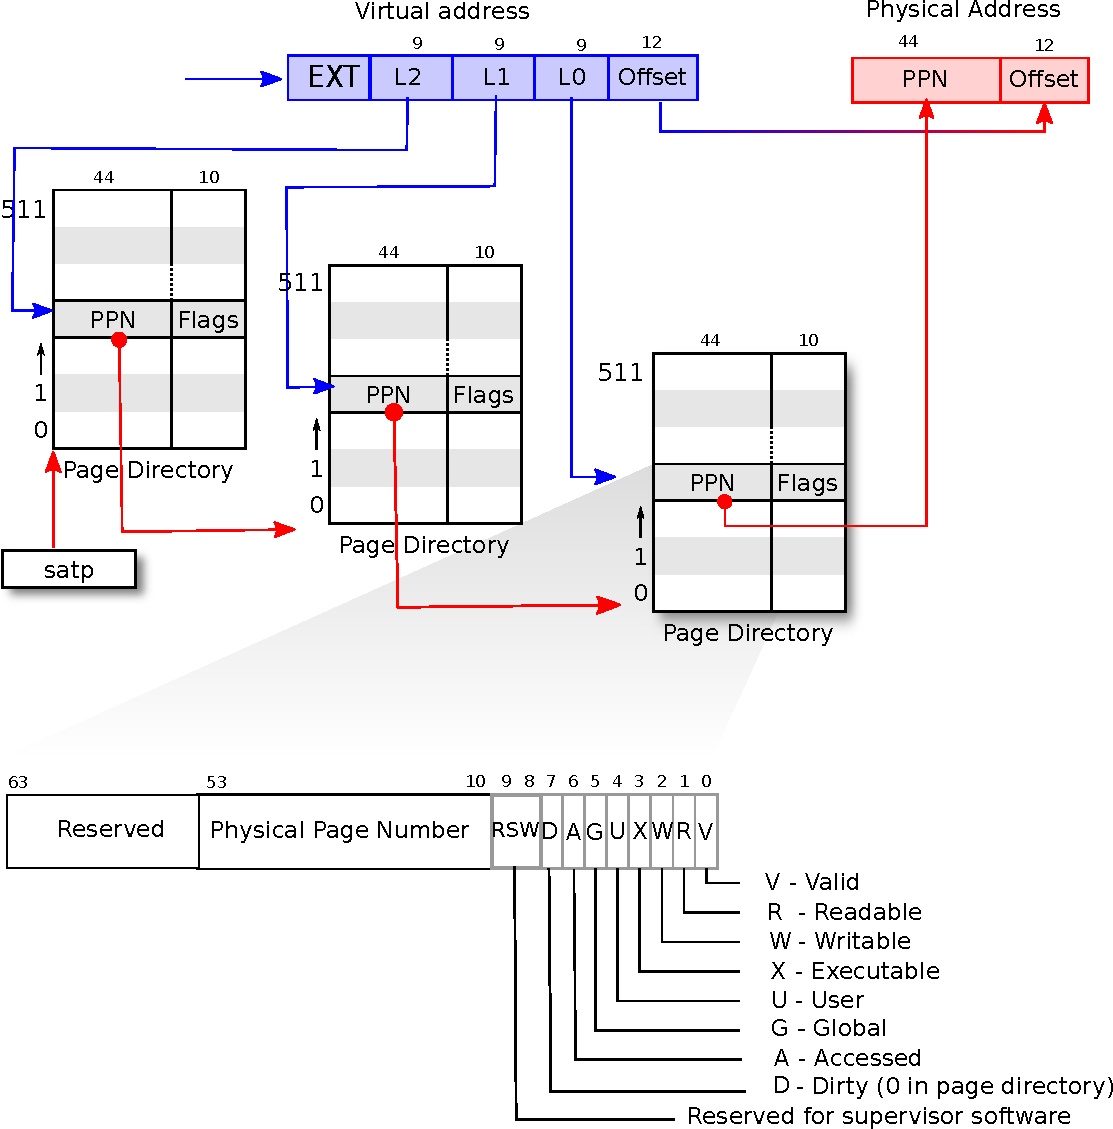
\includegraphics[scale=0.5, clip, trim=0cm 8cm 0cm 0cm]{riscv_pagetable.pdf}
    \end{center}

    © MIT \url{https://github.com/mit-pdos/xv6-riscv-book/}
  \end{frame}

\end{document}
